\chapter{Hardware Safety and Interlock Architecture}
\label{chap:safety}
% Traceability: ADR-001 ADR-003 ADR-004 ADR-005

The safety architecture follows one rule: a detected safety-related fault makes the controller safe through hardware. Software identifies and explains the cause afterward.

This order matters because the host, processor, FPGA, or acquisition clock may be part of the failure. None of them can be the only path that removes a hazardous detector-facing output.

The architecture starts from outputs that are safe when unpowered. It then combines several independent detection paths into one shared interlock. A fault on one board removes permission from every affected function board.

\section{Start at the Detector-Facing Output}

Detector protection relays are normally open. They require power and permission to energize. Loss of board power therefore opens the relay without waiting for software or firmware.

While power is available, a relay may energize only when these common conditions are true:

\begin{center}
\texttt{relay\_energized = local\_arm\_request AND EN AND OK}
\end{center}

The three conditions come from different parts of the system:

\begin{itemize}
  \item \texttt{local\_arm\_request} means the function board has completed its own readiness checks and deliberately requests operation;
  \item \texttt{EN} means the main board has armed the controller; and
  \item \texttt{OK} means no participant is currently asserting the shared hardware fault bus.
\end{itemize}

A board using active forwarding may add incoming-loop validity as another hardware permissive. Incoming LOOP LOW then removes local detector-facing permission without waiting for main, as described in Section~5.4.

Figure~\ref{fig:relay-permissive} shows the common permission path. The exact gate, latch, relay driver, and relay part are board-design choices. The required behavior is that loss of \texttt{EN}, \texttt{OK}, or local interlock power removes relay drive without depending on processor software, FPGA/CPLD state progress, or the distributed acquisition clock.

\begin{figure}[htbp]
  \centering
  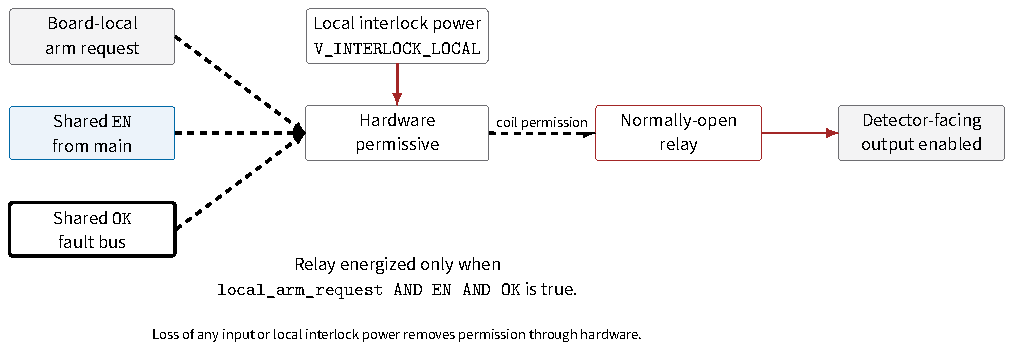
\includegraphics[width=0.92\textwidth]{figures/generated/relay_permissive.tikz.pdf}
  \caption{Common detector-facing hardware permissives; optional incoming-loop qualification is not shown. All required permissions must remain valid to energize a normally-open relay.}
  \label{fig:relay-permissive}
\end{figure}

Arming is therefore deliberate, while going safe is direct. A board cannot keep a detector protection relay energized merely because its FPGA still believes that it is in a running state.

\section{Three Safety Layers}

The complete system uses three cooperating layers. They have different response times and different dependencies.

\begin{table}[htbp]
\centering
\begin{tabularx}{\textwidth}{@{}>{\bfseries\raggedright\arraybackslash}p{0.22\textwidth}>{\raggedright\arraybackslash}p{0.34\textwidth}>{\raggedright\arraybackslash}X@{}}
\toprule
Layer & Main job & Important boundary \\
\midrule
Hardware interlock & Removes detector-facing permission when a shared or local trip occurs & Does not wait for host software or continued FPGA/CPLD operation \\
Board safety FSM & Checks readiness, retains fault evidence, controls local state, and coordinates recovery & Uses independent local management or safety clocking; FPGA or safety CPLD logic cannot override a hardware trip \\
Host management & Configures boards, coordinates instrument operation, and gathers diagnostics & Can request arm or recovery but cannot force hardware permission while a trip is active \\
\bottomrule
\end{tabularx}
\caption{The safety layers cooperate without giving software authority over the final hardware interlock.}
\label{tab:safety-layers}
\end{table}

The layers support one another. Hardware provides the fast and independent safe response. The board FSM keeps enough state for orderly operation and recovery. The host gives the operator a complete instrument view. Removing any one layer would either weaken protection or make the system difficult to operate and diagnose.

\section{The Shared Open-Drain Fault Bus}

The \texttt{OK} signal is a shared open-drain bus. The main board provides one pull-up. Every participating board and qualified backplane rail-health source may pull the bus low, but no function board drives it high.

Its meaning is intentionally simple:

\begin{itemize}
  \item \texttt{OK=1}: no participant is currently asserting the bus;
  \item \texttt{OK=0}: at least one participant is asserting a trip.
\end{itemize}

Because the bus is wired together, one fault removes permission across the controller. A board cannot mask another board's low assertion by driving high. The bus also remains useful when several sources trip at the same time.

The \texttt{OK} level does not identify the source. A healthy board enters its safe response when it sees the bus low, but it does not claim that it caused the trip. A board pulls the bus low only for its own retained local fault or supervisory event. After the safe response, the host reads diagnostics from the boards and common-rail measurements to find the cause.

This distinction prevents a fleet-wide trip from becoming a permanent loop in which every healthy board asserts its own fault output only because it observed \texttt{OK} low.

\section{The Continuity Loop}

The open-drain bus detects electronic faults, but it cannot by itself prove that every connector and cable remains present. A removed board cannot pull \texttt{OK} low. The architecture therefore adds a continuity loop.

The main board sends \texttt{LOOP\_OUT} through every slot and receives the returning signal as \texttt{LOOP\_IN}. Each board passes the path through passive copper or unconditional combinational hardware forwarding. Both types may coexist under the common electrical interface. It also passes through bridge cables and secondary backplanes when they are present.

If a board, passive terminator, connector, or extension cable opens the path, \texttt{LOOP\_IN} becomes invalid. Deterministic hardware on the main board converts that condition into its own \texttt{OK} assertion. Processor software is not the conversion path.

An unused slot contains a passive terminator that completes the loop. Removing an active board or terminator breaks the path and trips the system. This is intentional. Operational hot-swap is not supported.

During normal operation, active forwarding copies the incoming logic level independently of \texttt{OK}, \texttt{EN}, operating state, and clocks. On interlock-power loss it establishes LOW toward the next receiver. An output verified to become high impedance with an external pull-down is one implementation. The board may also make its outgoing loop LOW to report a detected condition that prevents its safety hardware from performing its role. Forwarding resumes when power and configuration are valid and that condition clears, without waiting for the retained trip to clear. Coverage of every possible internal device failure is not required. The complete chain must be valid before arming.

\begin{table}[htbp]
\centering
\small
\begin{tabularx}{\textwidth}{@{}l>{\raggedright\arraybackslash}X>{\raggedright\arraybackslash}X@{}}
\toprule
Implementation & Continuity & Interlock-power loss (F6) \\
\midrule
Passive copper & Direct connection & Separate hardware contribution to \texttt{OK} required \\
Active forwarding & Unconditional copy & Qualified LOW default propagates to main, which asserts \texttt{OK} \\
\bottomrule
\end{tabularx}
\caption{Permitted board continuity implementations. Empty-slot terminators remain passive.}
\end{table}

A function board using active forwarding may use incoming \texttt{LOOP\_IN} LOW to remove local detector-facing permission directly in hardware. This fast local response does not wait for main or a state-machine transition. LOW continues downstream to main, which asserts \texttt{OK} so every powered board, including those upstream of the fault, enters the shared safe response.

Local safe-state entry must not itself force the outgoing loop LOW. Forwarding remains independent of \texttt{OK}, \texttt{EN}, and operating state; it copies the input unless local power or a detected safety-hardware condition requires LOW. This avoids a recovery feedback loop. The chain propagates an upstream problem but does not automatically identify the affected board.

The backplane ICD defines loop voltage and logic thresholds, drive strength, leakage and loading, pull-down placement and values, unpowered and partial-power behavior, and total propagation time. Verification includes consecutive passive boards and terminators, configuration behavior, and prevention of back-powering. The architecture does not select a loop voltage.

Qualified active forwarding can provide F6 reporting without a separate local supervisor or hold-up supply. It does not prove that the rest of the CPLD is executing correctly and does not replace the watchdog. Main's own power-loss response needs a verified path independent of its failed conversion logic. A LOW return alone does not distinguish physical discontinuity (F1) from power loss in a forwarder (F6).

The continuity loop and \texttt{OK} bus solve different problems. The loop detects physical interruption and may also report interlock-power loss through qualified active forwarding. The open-drain bus carries electronic, timing, power, liveness, and supervisory trips. Both are required.

\section{Independent Fault Paths}

No single monitor can detect every important failure. The system uses several simple paths that converge on the shared \texttt{OK} bus. Figure~\ref{fig:fault-convergence} shows that convergence, and Table~\ref{tab:fault-paths} summarizes the main cases.

\begin{figure}[htbp]
  \centering
  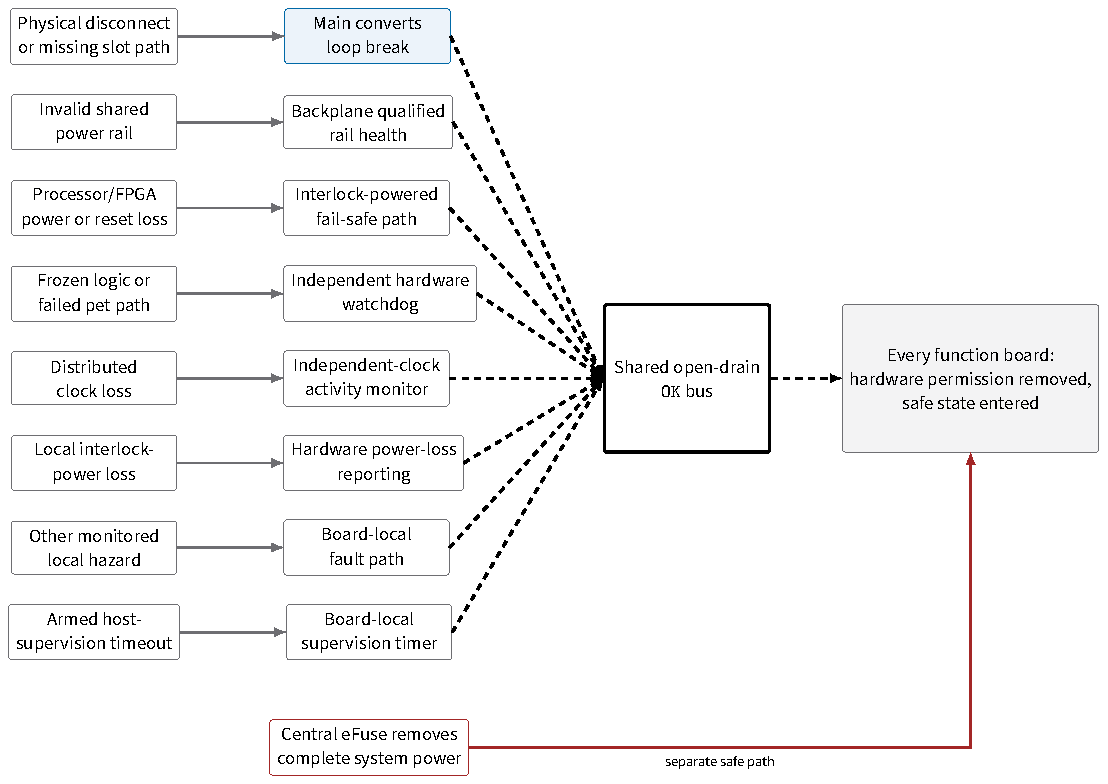
\includegraphics[width=\textwidth]{figures/generated/fault_convergence.tikz.pdf}
  \caption{Independent fault sources converge on the shared hardware trip and the same fleet-wide safe response. Complete central power removal is a separate safe path.}
  \label{fig:fault-convergence}
\end{figure}

\begin{table}[htbp]
\centering
\small
\begin{tabularx}{\textwidth}{@{}>{\bfseries\raggedright\arraybackslash}p{0.28\textwidth}>{\raggedright\arraybackslash}p{0.31\textwidth}>{\raggedright\arraybackslash}X@{}}
\toprule
Failure or event & Primary detection path & Safe propagation \\
\midrule
Physical disconnect or open slot path & Continuity loop, observed by main & Main pulls \texttt{OK} low \\
Invalid protected \texttt{+12V} or utility rail & Qualified backplane rail-health output & Backplane pulls \texttt{OK} low directly \\
Processor or FPGA rail loss or reset & Interlock-powered fail-safe circuit & Local hardware pulls \texttt{OK} low \\
Frozen logic or failed required pet path & Independent hardware watchdog & Watchdog path pulls \texttt{OK} low \\
Distributed acquisition-clock loss & Activity monitor running from an independent local clock & Board-local fault path pulls \texttt{OK} low \\
Loss of \texttt{V\_INTERLOCK\_LOCAL} on one board & Hardware power-loss reporting path & Hardware asserts the shared trip; local relay permission is removed \\
Other safety-related local condition & Board-specific monitor, where the hazard requires it & Board-local fault path pulls \texttt{OK} low \\
Loss of host supervision while armed & Board-local supervision timer & Timed-out board uses its normal local trip path \\
Complete central eFuse cutoff & Central input protection & All powered outputs and normally-open relays de-energize directly \\
\bottomrule
\end{tabularx}
\caption{Simplified mapping from representative failures to their protection paths.}
\label{tab:fault-paths}
\end{table}

The table does not mean that every local voltage needs a separate monitor. Additional local supervision is required only when an uncovered failure could leave a hazardous function active. Board hazard analysis determines those cases.

\section{Protection Must Survive the Failure It Detects}

The element that fails cannot also be the only means of detecting its failure.

\subsection{Power independent of the processor rails}

Each active board creates \texttt{V\_INTERLOCK\_LOCAL} from protected \texttt{+12V}. It powers the watchdog, fail-safe output, relay-permissive hardware, power-loss protection hardware, and any dedicated safety CPLD. It is separate from ordinary processor and acquisition-FPGA supplies.

If processor or FPGA power disappears, the interlock-powered fail-safe path treats loss of the active health signal as unsafe and asserts \texttt{OK}. If interlock power itself fails, its hardware power-loss path trips the powered fleet directly through \texttt{OK} or through qualified active loop forwarding and main, and the local relay releases. Complete system-power removal instead de-energizes powered hazards directly.

\subsection{A watchdog independent of the supervised clocks}

A powered but frozen processor or FPGA may leave a stale healthy output. The watchdog detects missing progress through its service signal, often called \emph{petting}. The processor or control logic refreshes it during normal execution; an autonomous toggle that continues after execution freezes is insufficient. Refresh timing uses local clocking and may optionally align to acquisition timing for noise control, with local fallback when that reference is absent.

The watchdog timeout time base remains operational when supervised clocks stop. A watchdog inside the supervised processor or FPGA may add coverage, but cannot replace this independent path. Clock-activity monitoring likewise uses independent local management or safety clocking.

\subsection{Implementing the functions with a safety CPLD}

A dedicated watchdog IC or a dedicated safety CPLD may implement the watchdog. A safety CPLD may also combine fault aggregation and retention, clock monitoring, main-board continuity-loop conversion, relay permissive logic, and evaluation of voltage/current-monitor indications. Analog sensing still needs suitable circuitry. The hardware F6 reporting path must remain effective when interlock power fails; a dedicated supply supervisor is optional.

The term \emph{safety CPLD} describes the device's assigned role, not a certification. A watchdog inside that CPLD does not independently cover failure of the same device. Board design addresses its power, reset, configuration, clock, and stale-permission failures, with bounded safe response and relay de-energization independent of continued logic progression. Figure~\ref{fig:safety-implementations} shows two possible implementations.

\begin{figure}[htbp]
  \centering
  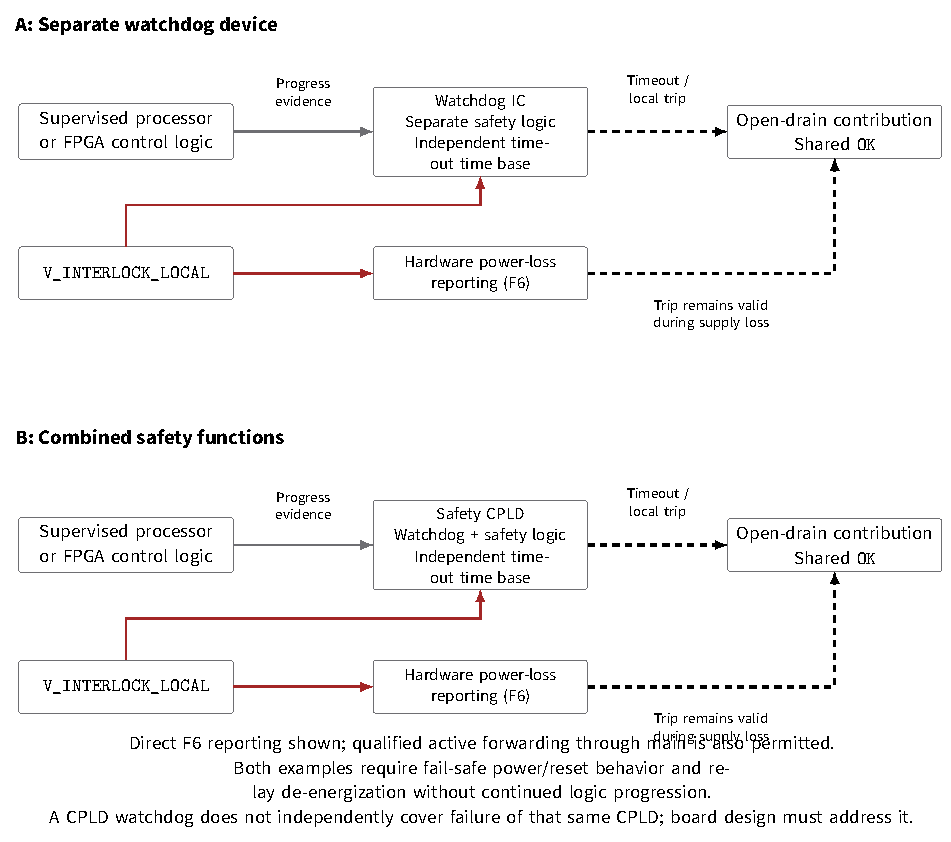
\includegraphics[width=\textwidth]{figures/generated/safety_implementations.tikz.pdf}
  \caption{Alternative implementations of the same safety functions. Both preserve independent watchdog timing and safe failure behavior. Direct F6 reporting is shown; qualified active loop forwarding is another permitted F6 path.}
  \label{fig:safety-implementations}
\end{figure}

\section{Safe First, Diagnose Second}

The clock monitor and watchdog report separate failures. Acquisition-clock loss enters the clock-monitor trip path. Missing processor/control-logic refreshes instead cause watchdog timeout. Either path can make the system safe before host diagnosis.

Each board retains local evidence that helps the host distinguish events after the trip. Clock-loss evidence is separate from watchdog activation. A responding board can report whether it detected a local fault, a host-supervision timeout, or only the shared trip from another participant. Main retains evidence of a broken continuity loop. Common-rail measurements help identify a power fault.

Watchdog activation directs investigation to processor/control-logic execution and its refresh path, separately from acquisition-clock loss. Communication silence alone establishes only that the board is unreachable, not that its power or logic has failed. Some severe failures leave a board unable to communicate. The host then combines the missing response with the hardware trip and the reports from the remaining boards. Diagnosis may be less precise, but the safe response does not depend on diagnostic completeness.

\section{Trips Remain Latched Until Explicit Recovery}

Restoring a clock, rail, temperature, or communication link does not release a retained trip. The host must request recovery, followed by live-condition qualification and a new arm request. Chapter~\ref{chap:lifecycle} explains the sequence.

\section{Finding a Damaged Fault-Output Path}

An open-drain fault driver can fail open. In that condition, the board may appear healthy during normal operation but fail to pull \texttt{OK} low when later needed. The continuity loop does not detect this electronic failure.

The system therefore supports a maintenance action that commands one selected board to assert its \texttt{OK} path while the host verifies that the shared bus changes state. The independent hardware watchdog path is also tested safely. Tests remain safely disarmed and demonstrate that the selected contribution causes an observable HIGH-to-LOW transition. A bus already held LOW by another source makes the assertion test inconclusive. Active protection is never bypassed to obtain a baseline.

The system ICD and maintenance plan define commands, schedule, acceptance timing, and service procedure.

Figure~\ref{fig:ok-maintenance-test} illustrates the observable test behavior without fixing command names or timing values. Release follows the defined safe test/recovery behavior; full system recovery is not necessarily needed solely to release a test contribution. Real fault retention and recovery still apply. Testing one contribution does not validate every independent watchdog or supervisor path.

\begin{figure}[htbp]
  \centering
  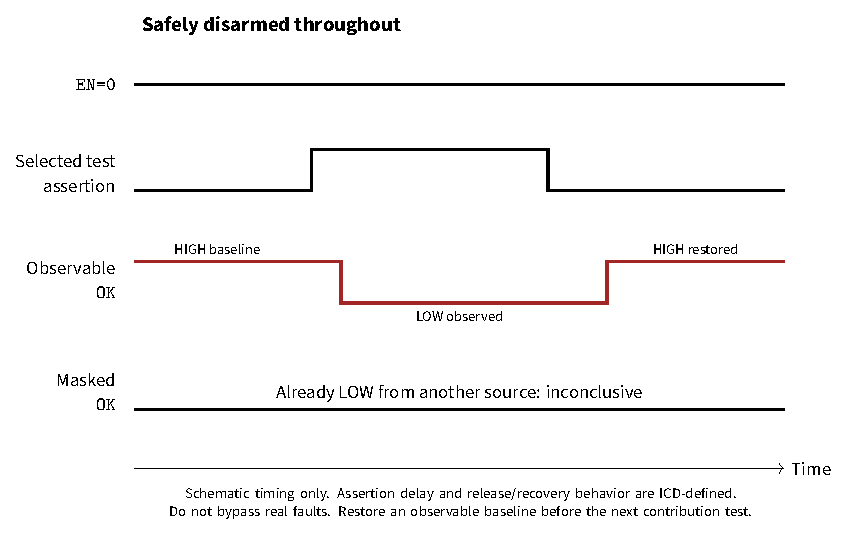
\includegraphics[width=0.95\textwidth]{figures/generated/ok_maintenance_test.tikz.pdf}
  \caption{Conclusive and masked assertion tests while safely disarmed. Time is schematic; acceptance intervals and safe test/recovery sequencing belong to the ICD and maintenance plan.}
  \label{fig:ok-maintenance-test}
\end{figure}

\section{Safety Scope}

The shared interlock provides a common response to detected faults. It does not prove that every possible detector hazard has been identified. Each function-board design still needs a hazard analysis for its detector-facing voltages, clocks, stored energy, output sequencing, and failure modes.

The architecture does not select watchdog parts, relay types, voltage thresholds, hold-up components, FPGA latches, or diagnostic registers. It also does not claim a formal safety integrity level. Those choices and claims require board-level analysis, verification, and any project-specific certification process.

The value of the architecture is a clear safety boundary: detector-facing permission is normally absent, independent hardware can remove it, all boards share the safe response, and software cannot override an active trip.

\medskip
\noindent\textit{Chapter sources:} ADR-001 defines the fault classes and independent detection paths. ADR-003 defines the safety layers, relay permissive, trip retention, and recovery rules. ADR-004 defines independent clock monitoring, and ADR-005 defines shared-rail fault reporting.
